\documentclass[convert={outfile=\jobname.png}]{standalone}
\usepackage{draw}
\usepackage{pgfgantt}

\begin{document}

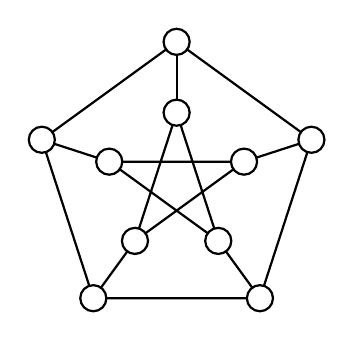
\begin{tikzpicture}[style=thick, scale=.9]
    \draw (18:2cm) -- (90:2cm) -- (162:2cm) -- (234:2cm) --
    (306:2cm) -- cycle;
    \draw (18:1cm) -- (162:1cm) -- (306:1cm) -- (90:1cm) --
    (234:1cm) -- cycle;
    \foreach \x in {18,90,162,234,306}{
            \draw (\x:1cm) -- (\x:2cm);
            \node[draw, circle, fill=white] at (\x:2cm) {};
            \node[draw, circle, fill=white] at (\x:1cm) {};
        }
\end{tikzpicture}

\end{document}
